\documentclass[11pt]{article}
\usepackage[top=1in, bottom=1in, left=1in, right=1in]{geometry}
\usepackage{hyperref}
\usepackage{graphicx}
\usepackage{subcaption}
\title{PHSX815 Project 1}
\author{Derek Grove}

\begin{document}
\maketitle
\subsection*{Introduction}
For this project I will be simulating an electron-positron collision at a specified collision energy. You will be able to configure what collision energy you want and how many experiments you want to run then the program will calculate which final-state products are allowed based on their rest masses. This is a toy model, the interaction is simplified by ignoring any higher order contributions or QFT nuances, I only consider an s-channel process. 

\begin{figure}[h!]
    \centering
    \begin{subfigure}[b]{0.4\linewidth}
      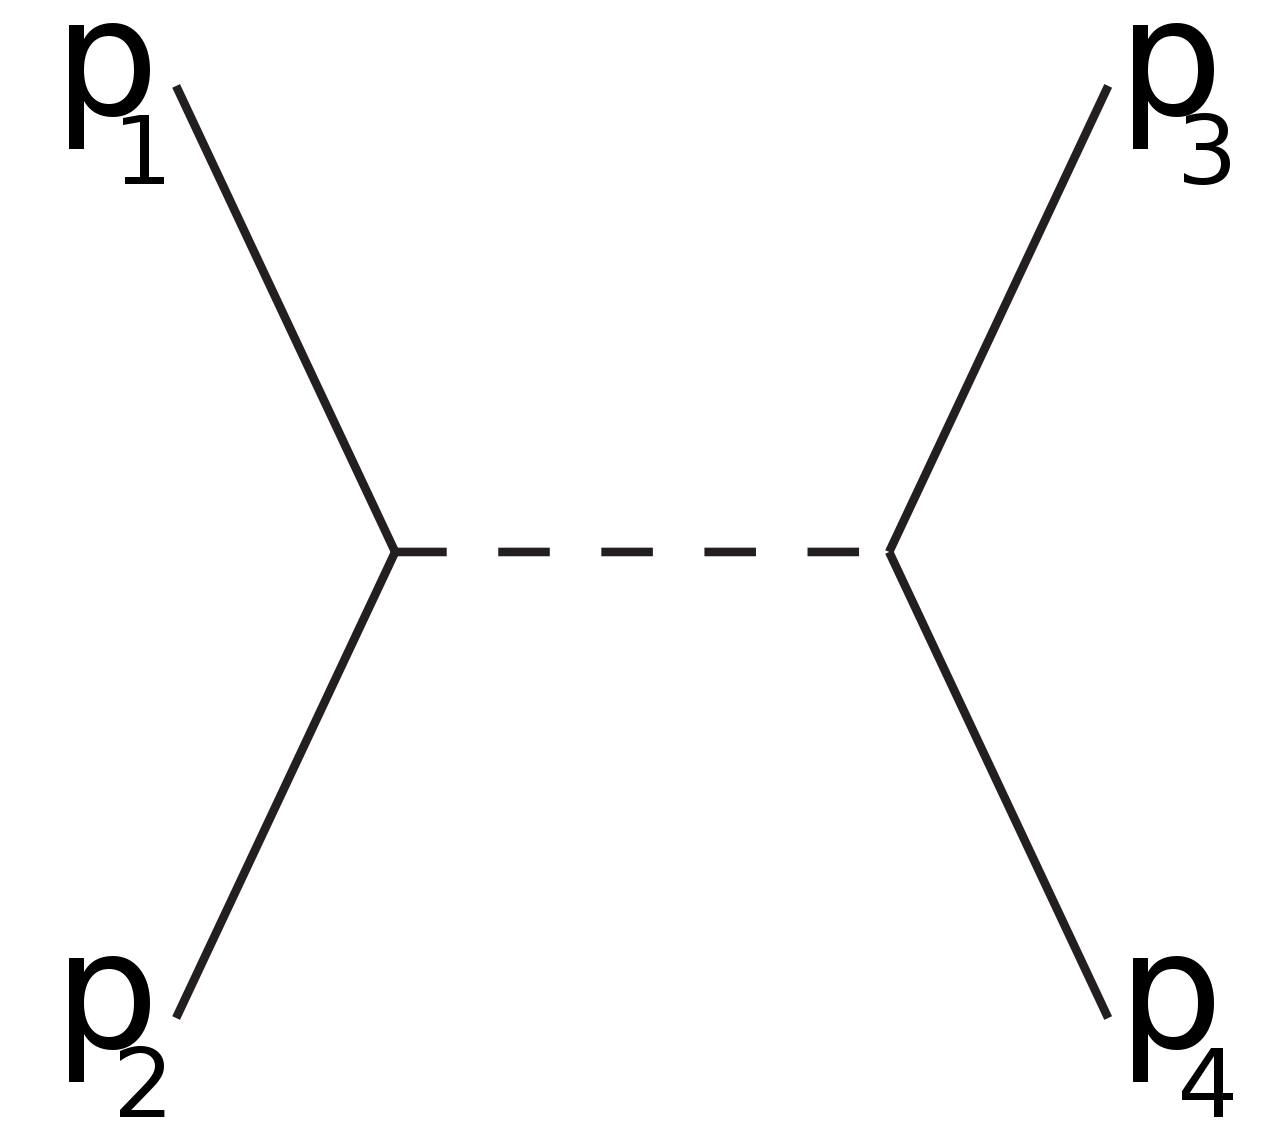
\includegraphics[width=130px]{Schannel.png}
    \end{subfigure}
    \caption{In my simulation, p1 = electron, p2 = positron, boson (dotted line) = photon}
    \label{fig:s-channel process}
  \end{figure}
  \vspace{1px}

Since the initial state is neutral (total charge = 0) the final states must also have zero net charge, so our possible products are all six leptons paired with their anti particle: $\nu_e\bar{\nu_e}$, $\nu_\mu\bar{\nu_\mu}$, $\nu_\tau\bar{\nu_\tau}$, $ee^+$, $\mu\bar{\mu}$, $\tau\bar{\tau}$, and then all 6 quarks paired with their anti particle: $u\bar{u}$, $d\bar{d}$, $c\bar{c}$, $s\bar{s}$, $t\bar{t}$, $b\bar{b}$. So, in figure 1, $p_3$ and $p_4$ are one of the above listed pairs. Which particles are allowed as final state products only depends on the initial state's collision energy. This is a categorical distribution with equal probability for each outcome. When it comes time to analyze the data I will hypothesize that this simulated decay prefers leptons over quarks, and I will (hopefully) be able to show that is not the case with my analysis code.

\subsection*{Algorithm Analysis}
For the simulation code, I first initialize the default collision energy and the number of experiments. I also initialize a vector of strings, call it product\_names, and fill it with (by order of ascending mass) the decay products possible from my above list. E-neutrino, mu-neutrino, so on and so forth. Since I'm explicitly defining this array I might as well save myself a step and sort it now. I then define an int named name\_size, set that equal to the product\_names array length. I then add a block that I copied from Chris Rogan's code to parse our command line and check for two key strings: "-Ce" and "-Nexp" and whatever ints follow them. This block is so I can pass this simulation different values of collision energy and/or number of experiments in the future. 

I then initialize another array, this time of doubles, and name it product\_masses. This array is also organized by way of increasing mass size, such that product\_name[0] corresponds to product\_mass[0], so on and so forth. Now, I finally do the calculation of which products are allowed. I first initialize a global variable called possible\_products\_size and a global int j. then, in a while loop, while j is less than the size of our product array (names\_size), I check if collision energy is greater than or equal to 2 times the product mass of product\_masses[j]. If Ce is greater than or equal to the mass of product\_masses[j], then I increment possible\_products\_size by 1, then regardless of the outcome I increment j by 1. This while loop runs until j is as long as our product\_names array (which is also the length of my product\_masses array). When that is complete, I now know how many products are possible, everything from product\_masses[0] up to product\_masses[possible\_products\_size]. 

Now, I would like to create a new array of only my possible products. I define an array possible\_products of length possible\_products\_size. I then use a for loop to iterate through the product\_masses array and fill possible\_products with those values, again maintaining the order of ascending mass. Now, the simulation is as easy as rolling a dice and comparing the outcome to an evenly split distribution. To create the distribution I divide 1.0 by possible\_products\_size and store that as a double named distribution. I am expecting a number for distribution like .25 or .3333333, etc. Next I define a seed by using a block of code I found online for a high precesion clock (it uses your computer's clock in units of nanoseconds to get very unique seeds. The regular method of using time(0) was not giving unique enough seeds when run back to back). I then feed that seed into srand, this is a required step when using the random functions in the standard c++ libraries. Finally, I use a for loop do "roll the dice" and print the outcome as many times as you define with Nexp. The rand() function outputs a number between 0 and 1, then I divide that number by distribution to determine which domain it falls into in my probability distribution. For example how this works, if we have 4 possible outcomes our distribution is 0 $\rightarrow$.25, .25$\rightarrow$.50, .50$\rightarrow$.75, .75$\rightarrow$1.0. Any number that falls between 0 and .25 should correspond to outcome 0, between .25 and .5 corresponds to outcome 1, and so on. So, a very easy way to check a random number and match it to the proper outcome is to divide your outcome by the value you are partitioning your distribution by, in the above example that would be .25. Whatever your outcome from the division is tells you the exact outcome that corresponds to (when indexing the outcome from 0, that is important). 

Making use of this quick check trick, I then just output the result of that division as the outcome of the simulation. To get the actual particle name you pass outcome into the particle\_names array and it will tell you the particle name. I left it as integer outputs to make the analysis easier, it'll be easier to have a .txt file full of ints rather than strings. 



\end{document}